\begin{boiboiboite}
	\propeau
	\propair
\end{boiboiboite}

\subsubsection{Cycle de Rankine}
	\label{exo_porcheville_rankine}

\begin{comment}
	1.800 tonnes/heure
	Fioul 10×plus cher que le charbon (1000 euros/tonne vs 100 euros)
	Chaque chaudière, 545° 180 bar, 130t fioul/heure
	Pression entrante turbines 150 bars
	Température de l’eau vers la seine: 3°C
	
	Charbon environ 35 MJ/kg
	
\end{comment}

	La centrale EDF de Porcheville (\cref{fig_porcheville}), en bordure de l’A13 à Mantes-la-Jolie, reçoit de la chaleur issue de la combustion de fioul, et utilise un cycle à vapeur pour alimenter une génératrice électrique.
	
	\begin{figure}
		\begin{center}
			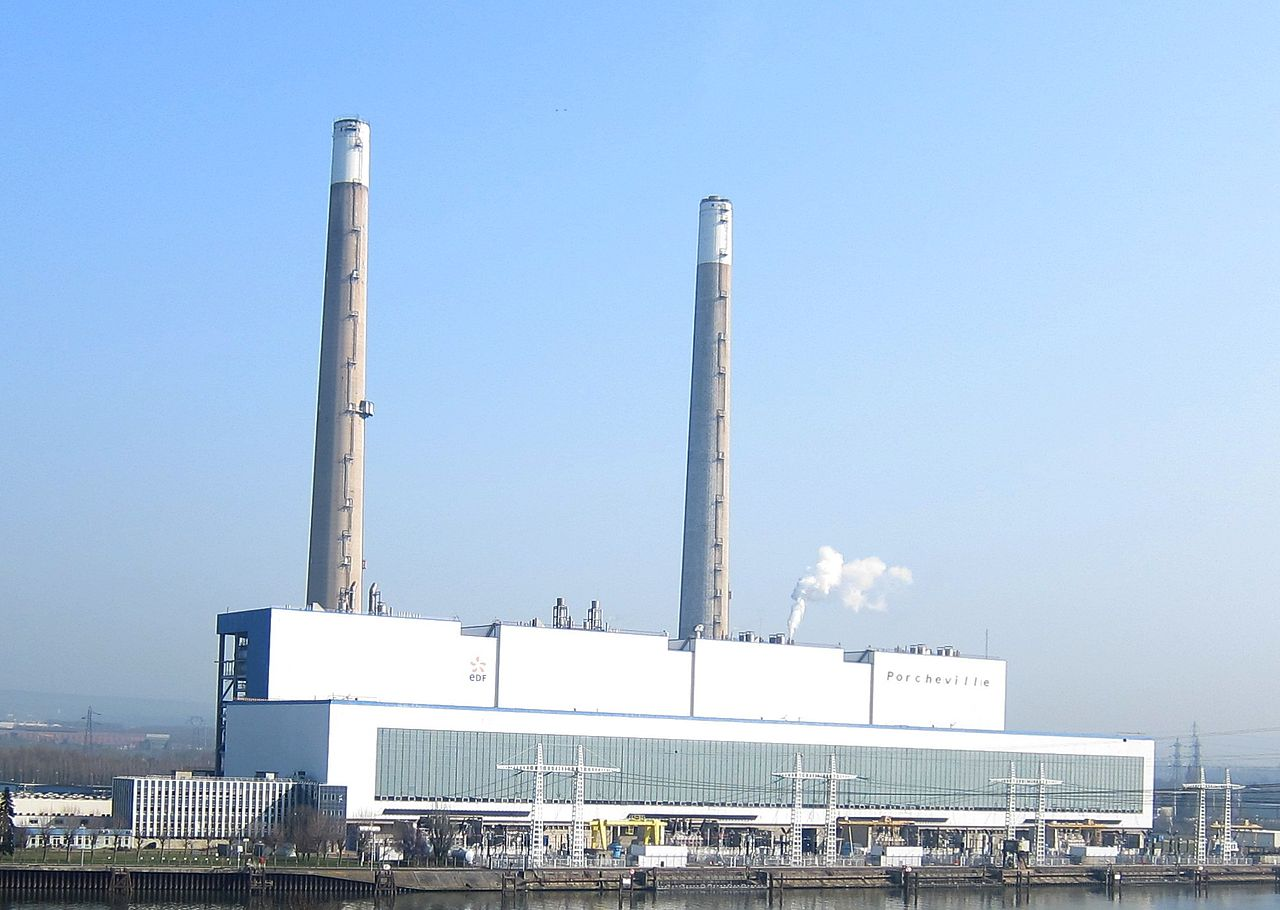
\includegraphics[width=8cm]{images/porcheville.jpg}
			\vspace{-0.5cm}
		\end{center}
		\supercaption{Centrale électrique de Porcheville, alimentée au charbon jusqu’en 1987 et fonctionnant désormais au fioul. Elle sert principalement les demandes de pointe.}{Photo schéma \cczero \oc}
		\label{fig_porcheville}
	\end{figure}
	
	Dans la centrale l’eau évolue entre les pressions de~\SI{0,1}{\bar} et~\SI{140}{\bar}. La vapeur atteint~\SI{545}{\degreeCelsius}, et les turbines ont une efficacité isentropique de~\SI{80}{\percent}.

	Dans cet exercice, nous considérons que le cycle est basé sur un cycle de Rankine surchauffé.
	
	\begin{enumerate}
		\item Schématisez le circuit physique de l’eau dans la centrale ; tracez le cycle suivi sur un diagramme température-entropie.
		\item Quelle est l’enthalpie spécifique de l’eau à la sortie de la turbine ?
		\item Quelle est l’enthalpie spécifique de l’eau à la sortie des pompes ?
		\item	Quel est le rendement thermodynamique de l’installation ?
		\item Quelle est la consommation spécifique de l’installation, c’est-à-dire la masse de vapeur ayant traversé la turbine lorsque l’installation a généré \SI{1}{\kWh} d’énergie mécanique ?
		\item Quel débit horaire de vapeur faut-il faire circuler dans le circuit pour obtenir une puissance mécanique de~\SI{60}{\mega\watt} ?
	\end{enumerate}
	

\subsubsection{Chaudière de centrale à vapeur}

	Dans une centrale à vapeur, la chaudière fonctionne avec la combustion de bois dans de l’air prélevé dans l’atmosphère. Les briquettes utilisées pour la combustion sont faites de résidus de bois et de biomasse (\cref{fig_sciure}) ; elles ont une capacité calorifique massique de~\SI{15}{\mega\joule\per\kilogram}.
	
	\begin{figure}
		\begin{center}
			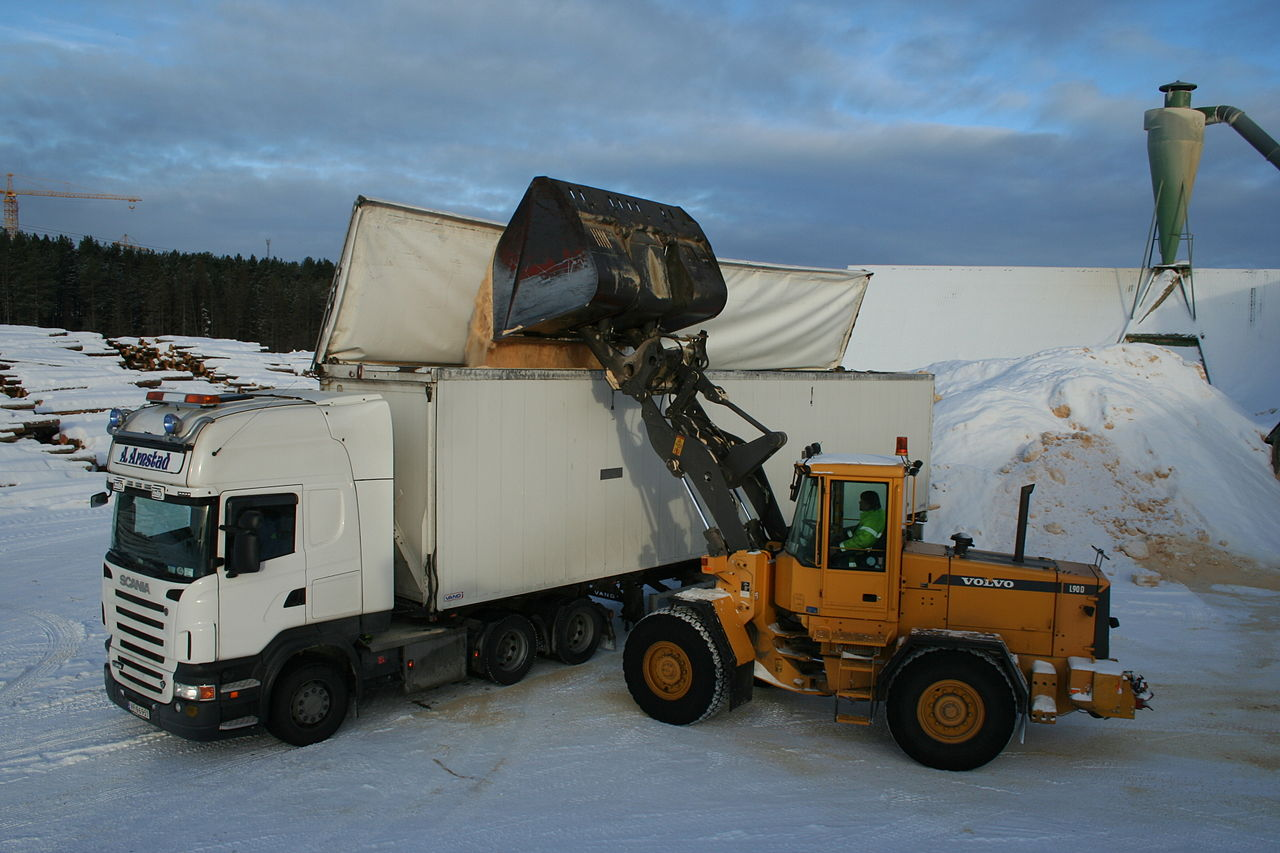
\includegraphics[width=8cm]{images/sciure.jpg}
		\end{center}
		\supercaption{La sciure de bois, produite en très grande quantité dans l’industrie, peut être utilisée comme source d’énergie dans une centrale à vapeur.}{\wcfile{Flislasting.jpg}{Photo} \ccbysa par \wcu{Eivindmy}}
		\label{fig_sciure}
	\end{figure}
	
	L’air pénètre dans la chaudière à température de~\SI{15}{\degreeCelsius} et pression de~\SI{1}{\bar}. Il est porté à température de~\SI{1000}{\degreeCelsius} par combustion à pression constante, avant de passer autour des conduits d’eau.	Lorsqu’il quitte la chaudière, sa température est de~\SI{180}{\degreeCelsius}.

	L’eau pénètre dans la chaudière à~\SI{50}{\bar} et~\SI{20}{\degreeCelsius}. Elle y circule à pression constante. On souhaite la porter jusqu’à une température de~\SI{850}{\degreeCelsius}, avec un débit de~\SI{3}{\kilogram\per\second}.
	
	\begin{enumerate}
		\item Quel débit d’air faut-il admettre dans la chaudière pour respecter le cahier des charges ?
		\item Quelle est l’efficacité de la chaudière ?
		\item Un/e ingénieur/e propose de faire passer le conduit d’air d’admission au travers des gaz d’échappement (sans pourtant les mélanger) pour augmenter la température de l’air avant combustion. Cela vous paraît-il être une bonne idée ?
	\end{enumerate}


\subsubsection{Cycle avec resurchauffe}

	L’installation de Porcheville décrite dans l’exercice~\ref{exo_porcheville_rankine} est modifiée pour accueillir une série de tubes de resurchauffe. La détente de l’eau est interrompue à~\SI{18}{\bar} dans la turbine, et la vapeur est ramenée à la température maximale du cycle (c’est-à-dire \SI{545}{\degreeCelsius}).
	
	La centrale est alimentée au fioul lourd dit «~TBTS~», de masse volumique \SI{1050}{\kilogram\per\metre\cubed} et de pouvoir calorifique \SI{40,2}{\mega\joule\per\kilogram}. La chaudière a une efficacité de~\SI{80}{\percent}.
	
	\begin{enumerate}
		\item Quel est le nouveau rendement de l’installation ?
		\item Quelle est la nouvelle consommation spécifique ?
		\item Quel est le débit volumique horaire de carburant nécessaire pour générer \SI{60}{\mega\watt} électriques ?
	\end{enumerate}
	

\subsubsection{Cycle avec régénération}

	Dans un navire brise-glace polaire (\cref{fig_50letpodeby}), une installation à vapeur alimente les hélices à partir d’un réacteur nucléaire.

	\begin{figure}
		\begin{center}
			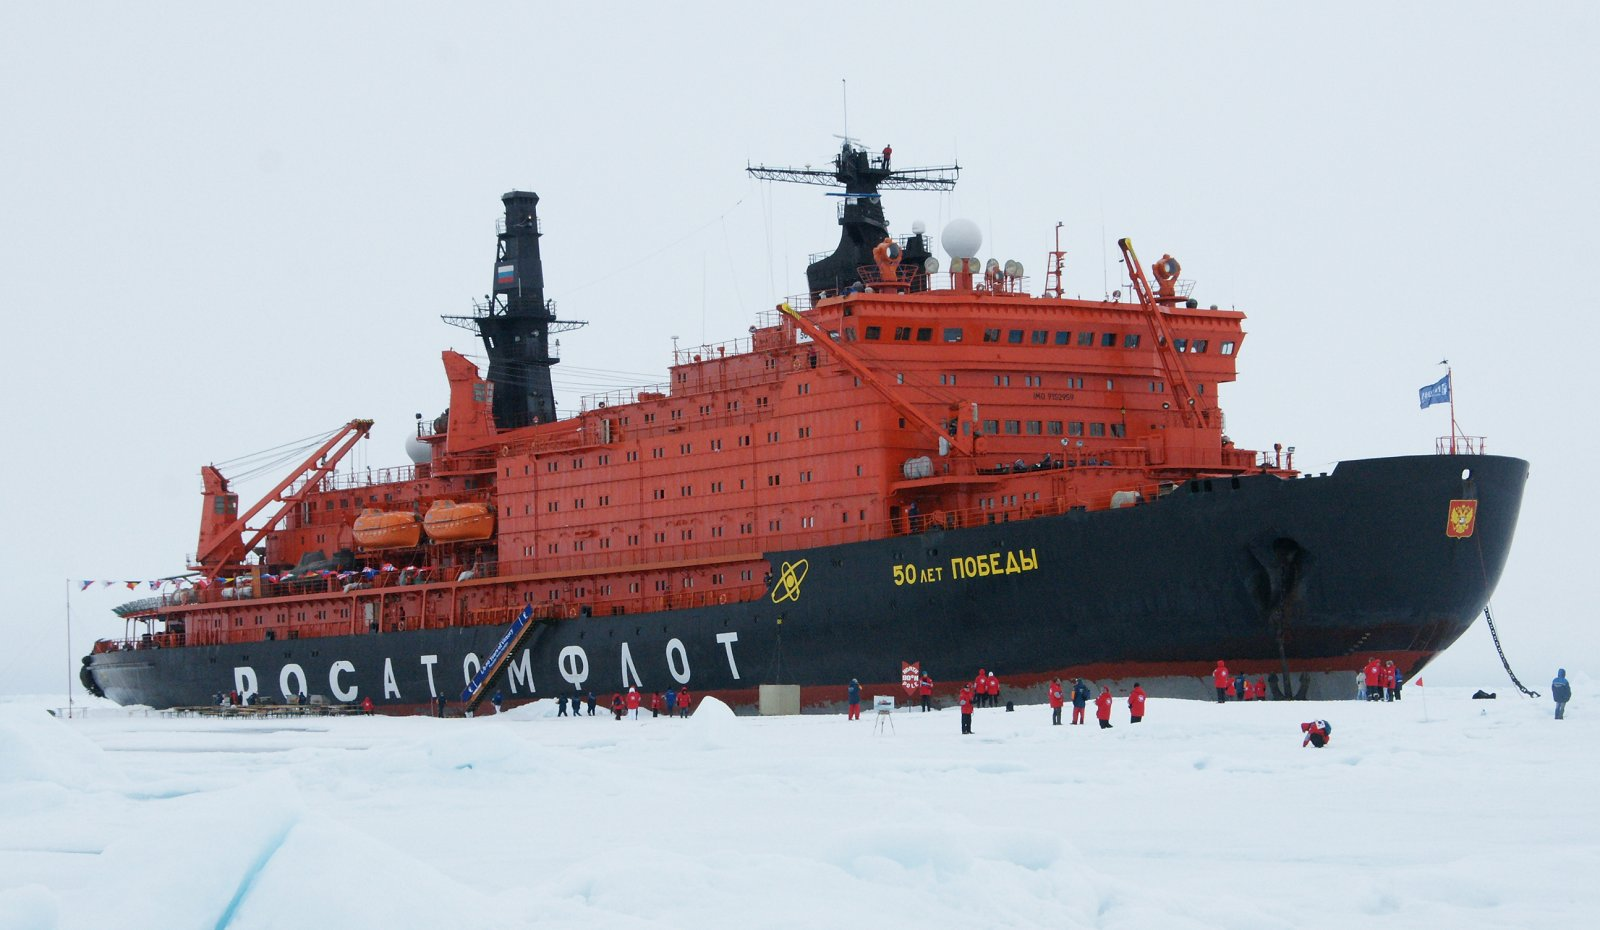
\includegraphics[width=11cm]{images/50letpodeby.jpg}
		\end{center}
		\supercaption{Le 50 Let Podeby, brise-glace de~\SI{25 000}{\tonne} à propulsion nucléo-turbo-électrique (deux réacteurs de~$\SI{171}{\mega\watt}_{\text{chaleur}}$, trois moteurs de~$\SI{17,6}{\mega\watt}_{\text{méch.}}$). Sa construction a débuté en 1989 mais il n’est entré en service qu’en 2007.}{\wcfile{50letPob_pole.JPG}{Photo} \ccbysa par \wcu{Kiselev d}}
		\label{fig_50letpodeby}
	\end{figure}

	Le cycle est basé sur un cycle de Rankine surchauffé à~\SI{310}{\degreeCelsius} (par contact avec les conduites d’eau pressurisée qui, elle, traverse le réacteur), entre les pressions de~\num{30} et~\SI{0,5}{\bar}\footnote{En réalité, entre \num{29} et~\SI{0,75}{\bar}, valeurs qui ne sont pas tabulées dans nos abaques.}. Nous considérons que la turbine est parfaitement isolée et isentropique.% en réalité, 29 et 0,75 bar

	\begin{enumerate}
		\item Quel est le rendement thermodynamique de l’installation ?
		\item On définit la consommation spécifique de vapeur comme l’inverse de la puissance nette de l’installation. C’est la masse de vapeur ayant traversé la turbine lorsque l’installation a généré \SI{1}{\kWh} d’énergie mécanique.\\
			Quelle est la consommation spécifique de l’installation ?
	\end{enumerate}

	Un/e ingénieur/e propose de modifier le cycle pour le rendre régénératif, en prélevant de la vapeur de la turbine pour l’insérer dans le circuit de compression.
	
	Il/elle propose de séparer la compression en deux étapes, l’une de~\num{0,5} à~\SI{6}{\bar}, et la seconde de~\num{6} à~\SI{30}{\bar} ; et d’insérer la vapeur prélevée entre les deux pompes. Le débit de vapeur prélevé est tel que l’eau à la sortie du mélangeur est exactement à saturation.
	
	Pour alléger nos calculs, nous considérons que la puissance de pompage n’est pas modifiée par la régénération.
	
	\begin{enumerate}	
		\shift{2}
		\item Schématisez l’installation proposée (c’est-à-dire le circuit physique suivi par la vapeur).
		\item Représentez le cycle thermodynamique sur un diagramme température-entropie, en traçant la courbe de saturation de l’eau.
		\item Quelle proportion du débit de vapeur faudrait-il prélever à~\SI{6}{\bar} dans la turbine, pour chauffer l’eau à saturation entre les deux pompes ?
		\item La puissance aux hélices augmente-t-elle ou diminue-t-elle, et de combien ?
		\item Le rendement de l’installation augmente-t-il ou diminue-t-il, et de combien ?
	\end{enumerate}

\exercisesolutionpage
\subsubsection*{Résultats}
	\linktosolutionsblurb
	
	\begin{description}
		\item [9.1] \tab 2) $h_\D = \SI{2287,7}{\kilo\joule\per\kilogram} $ 
						\tab 3) $h_\B = \SI{205,9}{\kilo\joule\per\kilogram} $ 
						\tab 4) $\eta_\text{inst.} = \SI{35,29}{\percent}$ 
						\tab 5) $SSC = \SI[per-mode = symbol]{3,15}{\kilogram\per\kilo\watt\per\hour}$ 
						\tab 6) $\dot{m}_\text{eau} = \SI{52,5}{\kilogram\per\second}$
		\item [9.2] \tab 1) $\dot{m}_\text{air} = \SI{15,2}{\kilogram\per\second}$ 
						\tab 2) $\eta_\text{chaud.} = \SI{83,25}{\percent}$
		\item [9.3] \tab 1) $h_{D2} = \SI{2960,8}{\kilo\joule\per\kilogram}$, $h_{E2} = \SI{3570,3}{\kilo\joule\per\kilogram}$, $h_{F} = \SI{2642,7}{\kilo\joule\per\kilogram}$ : $\eta_\text{inst.2} = \SI{36,31}{\percent}$ (\SI{+1}{pt})
						\tab 2) $\dot{V}_\text{carb.} = \SI{17,6}{\metre\cubed\per\hour}$.
		\item [9.4] \tab 1) $h_{A} = \SI{340,5}{\kilo\joule\per\kilogram}$, $h_{B} = \SI{343,54}{\kilo\joule\per\kilogram}$, $h_{C} = \SI{3017,4}{\kilo\joule\per\kilogram}$, $h_{D} = \SI{2284,5}{\kilo\joule\per\kilogram}$ : $\eta_\text{inst.} = \SI{27,294}{\percent}$. 
						\tab 2) $SSC = \SI[per-mode = symbol]{4,93}{\kilogram\per\kilo\watt\per\hour}$ 
						\tab 5) $h_\text{prélèvement} = \SI{2673,9}{\kilo\joule\per\kilogram}$, $h_\text{pré-mélange} = \SI{341,1}{\kilo\joule\per\kilogram}$, $h_\text{post-mélange} = \SI{670,4}{\kilo\joule\per\kilogram}$ : $z = \SI{14,1}{\percent}$
						\tab 6) $w_\text{net~2} = \SI{-674,87}{\kilo\joule\per\kilogram}$ (\SI{-9,2}{\percent}) 
						\tab 7) $q_\text{chaud.} = \SI{2344,4}{\kilo\joule\per\kilogram}$ : $\eta_\text{inst.~2} = \SI{28,786}{\percent}$ (\SI{+1,49}{pt})
	\end{description}
